\section{Function of the Central Dogma}
Up to this point, we have considered a variety of transport and biosynthetic
processes that are critical to acquiring and generating new cell mass. While
there are of course many other metabolic processes we could consider and
perform estimates of (such as the components of fermentative versus aerobic
respiration), we now turn our focus to some of the most central processes
which \textit{must} be undertaken irrespective of the growth conditions --
the processes of the central dogma.


\subsection{DNA}
Most bacteria (including \textit{E. coli}) harbor a single,
circular chromosome and can have extra-chromosomal plasmids $\sim$ 100 kbp in
length. We will focus our quantitative thinking solely on the chromosome of
\textit{E. coli} which harbors $\approx$ 5000 genes and $\approx 5\times
10^6$ base pairs. To successfully divide and produce viable progeny, this chromosome must be faithfully replicated and
segregated into each nascent cell. We again rely on the near century of literature in molecular biology to provide some insight
towards the rates and mechanics of the replicative feat as well as the
production of the replication starting materials, dNTPs.

\subsubsection{dNTP synthesis}
We begin our exploration of the DNA replicative processes by examining the
production of the deoxyribonucleotide triphosphates (dNTPs). The four major
dNTPS (dATP, dTTP, dCTP, and dGTP) are synthesized \textit{de novo} in separate
pathways, requiring different building blocks. However, a critical step present
in all dNTP synthesis pathways is the conversion from ribonucleotide to
deoxyribonucleotide via the removal of the 3' hydroxyl group of the ribose ring
CITE. This reaction is mediated by a class of enzymes termed ribonucleotide
reductases, of which \textit{E. coli} possesses two aerobically active complexes
(termed I and II) and a single anaerobically active enzyme CITE. Due to their
peculiar formation of a peculiar radical intermediate, these enzymes have
received much biochemical kinetic and structural characterization.  One such
work \citep{ge2003} performed a detailed \textit{in vitro} measurement of the
steady-state kinetic rates of these complexes, revealing a turnover rate of
$\approx$ 10 per second.

Considering this reaction (mediated by the ribonucleotide reductase complexes I
and II) is central to synthesis of all dNTPS, it is reasonable to consider the
abundance of these complexes as a measure of the total dNTP production in
\textit{E. coli}. Illustrated schematically in \FIG{dna_synthesis}(A), we
consider the fact that to replicate the cell's genome, on the order of $\approx
10^7$ dNTPs must be synthesized. Assuming a production rate of 10 per second per
ribonucleotide reductase complex and a cell division time of 6000 seconds, we
arrive at an estimate of $\approx$ 150 complexes are needed per cell. As shown
in the bottom panel of \FIG{dna_synthesis}(A), this estimate agrees with the
experimental measurements of these complexes abundances within $\approx 1/2$ an
order of magnitude. 

Recent work has that during replication, the ribonucleotide reductases complexes
localize into discrete foci colocalized with the DNA replisome complex
\citep{sanchez-romero2011}. This is particularly pronounced in environments
where growth is slow, indicating that spatial organization and regulation of the
activity of the complexes plays an important role. 

\begin{figure} 
    \begin{fullwidth} 
        \centering{
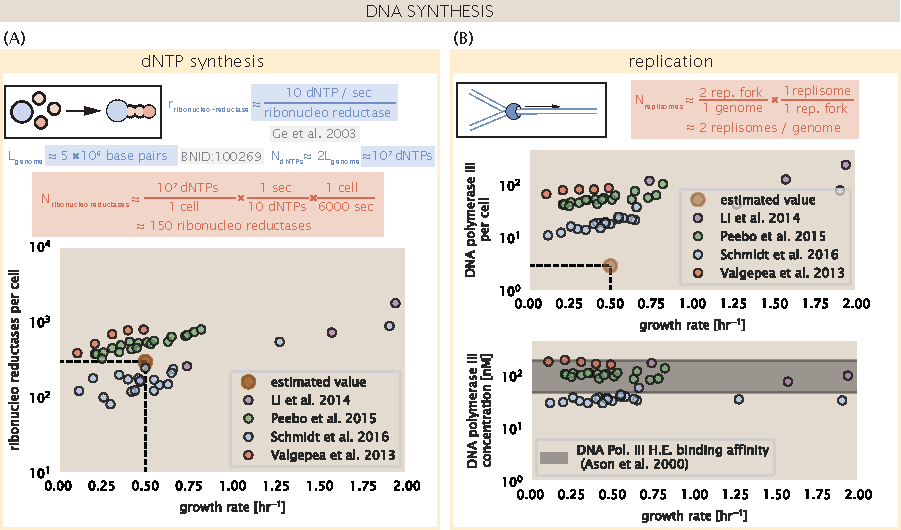
\includegraphics{main_figs/DNA_synthesis} \caption{\textbf{Complex abundance
estimates for dNTP synthesis and DNA replication.} (A) Estimate of the number
of ribonucleotide reductases enzymes needed to facilitate the synthesis of
$\approx 10^7$ dNTPs over the course of a 6000 second generation time. Points
in the plot correspond to the total number of ribonucleotide reductase I
([NrdA]$_2$[NrdB]$_2$) and ribonucleotide reductase II ([NrdE]$_2$[NrdF]$_2$)
complexes. (B) An estimate for the minimum number of DNA polymerases
holoenzyme complexes needed to facilitate replication of a single genome.
Points in the top plot correspond to the total number of DNA polymerase III
holoenzyme complexes
([DnaE]$_3$[DnaQ]$_3$[HolE]$_3$[DnaX]$_5$[HolB][HolA][DnaN]$_4$[HolC]$_4$[HolD]$_4$)
per cell. Bottom plot shows the effective concentration of DNA polymerase III
holoenzyme given cell volumes calculated from the growth rate as in
\cite{si2019}.} 
\label{fig:DNA_synthesis} } 
\end{fullwidth} 
\end{figure}


\subsubsection{DNA Replication}
We now turn our focus towards the process of integration of the dNTP building
blocks into the replicated chromosome strand via the DNA polymerase enzymes.
Replication of bacterial chromosomes is initiated at a single region of the
chromosome termed the \textit{oriC} locus at which a pair of DNA polymerases
bind and begin their high-fidelity replication of the genome in opposite
directions. Assuming equivalence between the two replication forks, this
means that the two DNA polymerases meet at the midway point of the circular
chromosome termed the \textit{ter} locus. This division of labor means The
kinetics of the four types of DNA polymerases (I -- V) have been intensely
studied, revealing that DNA polymerase III performs the high fidelity
processive replication of the genome with the other "accessory" polymerases
playing auxiliary roles \cite{fijalkowska2012}. \textit{In vitro}
measurements have shown that DNA Polymerase III copies DNA at a rate of
$\approx 600$ nucleotides per second (BNID: 104120, \cite{milo2010}). Thus,
to replicate a single chromosome, two DNA polymerases replicating at their
maximal rate would copy the entire genome in $\approx$ 4000 s. Thus, with a
division time of 6000 s (our "typical" growth rate for the purposes of this
work), there is sufficient time for a pair of DNA polymerases to replicate
the entire genome. However, this estimate implies that 4000 s would be the
upper-limit time scale for bacterial division which is at odds with the
familiar $\approx$ 1500 s doubling time of \textit{E. coli} in rich medium.

It is know well known that \textit{E. coli} can parallelize its DNA
replication such that multiple chromosomes are being replicated at once.
Recent work \citep{si2017} has shown that the replicative timescale of cell
division can be massively parallelized where \textit{E. coli} can have on the
order of 10 - 12 replication forks at a given time. Thus, even in rapidly
growing cultures, only a few polymerases ($\approx 10$) are needed to
replicate the chromosome. However, as shown in \FIG{dna_synthesis}(B), DNA
polymerase III is nearly an nearly an order of magnitude more abundant. This
discrepancy can be understood when considering the binding affinities. The
DNA polymerase III complex is highly processive, facilitated by a strong
affinity of the complex to the DNA. \textit{In vitro} biochemical
characterization has quantified the $K_D$ of DNA polymerase III holoenzyme to
single-stranded and double-stranded DNA to be 50 and 200 nM, respectively.
The bottom plot in \FIG{DNA_synthesis}(B) shows that the concentration of the
DNA polymerase III across all data sets and growth conditions is within this
range \citep{ason2000}. Thus, while the copy number of the DNA polymerase III
is in excess of the strict number required to replicate the genome, the copy
number is tuned such that the concentration is approximately equal to the
dissociation constant to the DNA. While the processes regulating the
initiation of DNA replication are complex and involve more than just the
holoenzyme, these data indicate that the kinetics of replication rather than
the explicit copy number of the DNA polymerase III holoenzyme is the more
relevant feature of DNA replication to consider.
